% ============================================================
%  Presentación — ¿Cómo estimar el índice de Theil con la GEIH?
%  Proyecto de Estadística (73210011), Universidad del Rosario, 2026-II
%
%  Las tablas y figuras vienen de outputs/ (las genera R con run_all.R).
%  Compilar desde esta carpeta: pdflatex -> biber -> pdflatex
%  Unos 12 a 15 minutos: una idea por diapositiva.
% ============================================================
\documentclass[aspectratio=169,10pt]{beamer}

\usepackage[T1]{fontenc}
\usepackage[utf8]{inputenc}
\usepackage[spanish,es-nodecimaldot,es-noshorthands]{babel}
\usepackage{newtxtext,newtxmath}
\usepackage{icomma}
\usepackage{booktabs}

\usetheme{default}
\setbeamertemplate{navigation symbols}{}
\setbeamertemplate{footline}[frame number]

\graphicspath{{../outputs/figuras/}{../docs/curso/report/}}
\newcommand{\tabla}[1]{\input{../outputs/tablas/#1.tex}}
\newcommand{\tablaancha}[1]{\resizebox{\textwidth}{!}{\tabla{#1}}}

\usepackage{csquotes}
\usepackage[backend=biber,style=apa]{biblatex}
\addbibresource{../report/references.bib}

\title{¿Cómo estimar el índice de Theil con la GEIH?}
\subtitle{Desigualdad del ingreso laboral en Colombia, 2018--2026}
\author{Gabriel Salcedo \and Jerónimo Marín \and Isaac Suarez \and Santiago Velandia}
\institute{Universidad del Rosario --- Estadística}
\date{Noviembre de 2026}

\begin{document}

\begin{frame}
  \titlepage
\end{frame}

% ------------------------------------------------------------
\begin{frame}{El problema}
  % Una frase: medir desigualdad con encuestas exige elegir un estimador.
  % La pregunta de investigación (CLAUDE.md, sección 3).
\end{frame}

\begin{frame}{Hipótesis}
  % H1, H2 y H3 en una línea cada una.
\end{frame}

% ------------------------------------------------------------
\begin{frame}{Datos: GEIH 2018--2026}
  % Fuente, población, n por año, por qué usar el factor de expansión.
\end{frame}

\begin{frame}{Cuatro estimadores del índice de Theil}
  % A, B, C y D: fórmula y supuesto de cada uno.
\end{frame}

% ------------------------------------------------------------
\begin{frame}{¿Cómo es el ingreso laboral?}
  \centering
  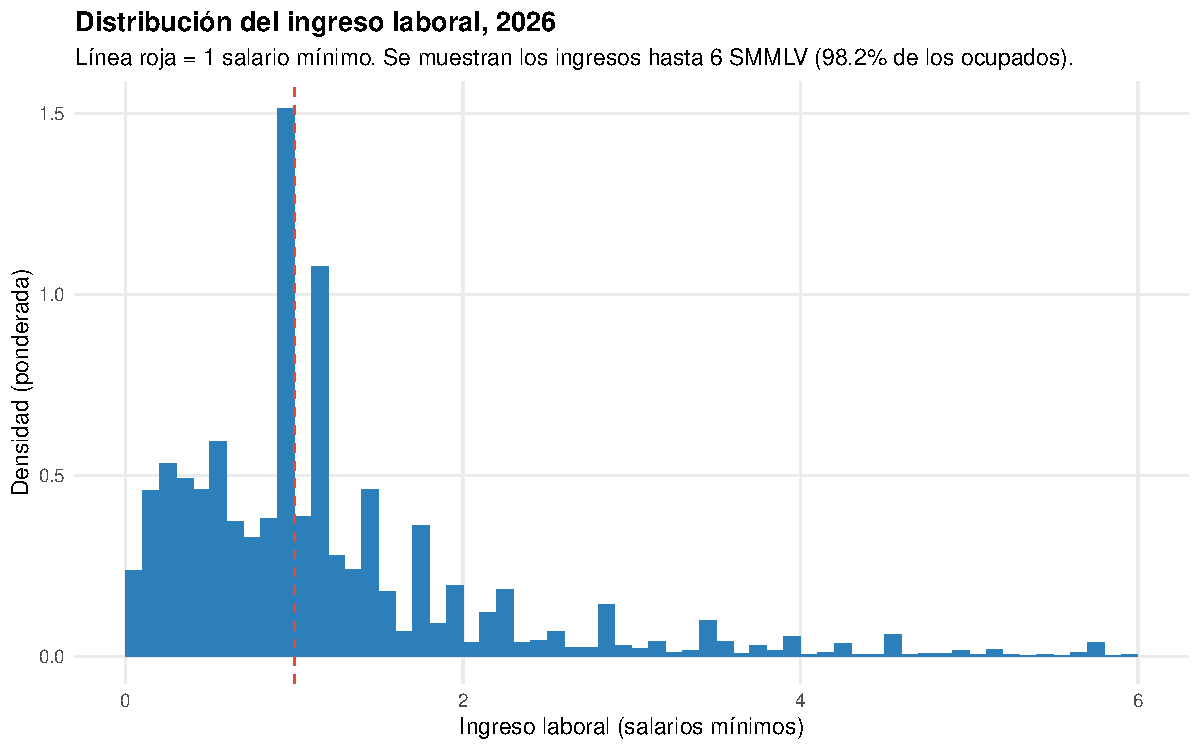
\includegraphics[height=0.8\textheight]{07a_histograma_ingreso}
  % Mensaje: pico en el salario mínimo.
\end{frame}

\begin{frame}{¿Es lognormal?}
  \centering
  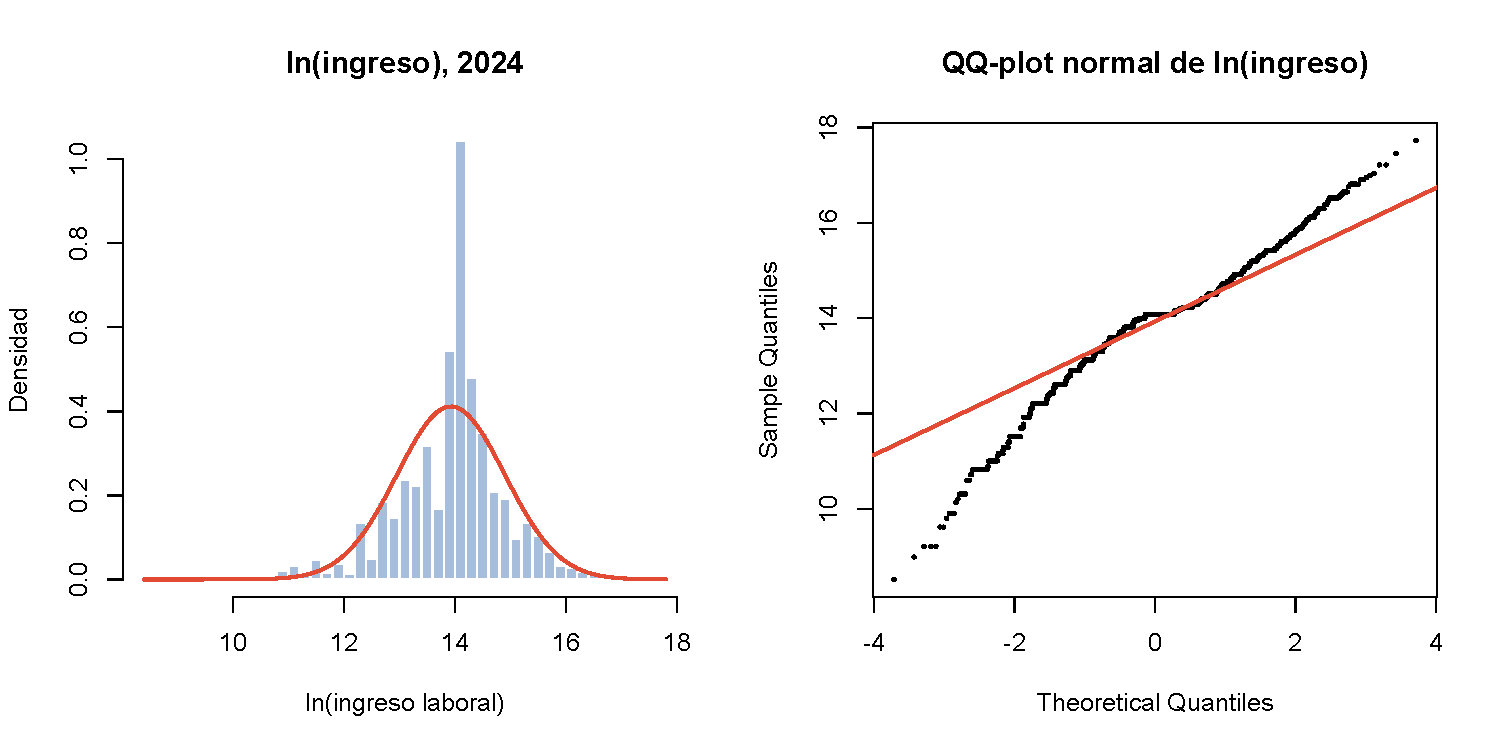
\includegraphics[width=\textwidth]{p7_ln_ingreso_normalidad}
  % Mensaje: no; por eso C y D deberían fallar.
\end{frame}

% ------------------------------------------------------------
\begin{frame}{Simulación Monte Carlo (H1)}
  % Diseño y resultado: tabla de ECM/ER o figura de ECM frente a n.
  % PENDIENTE: la simulación todavía no existe.
\end{frame}

% ------------------------------------------------------------
\begin{frame}{Desigualdad 2018--2026}
  \centering
  \tabla{theil_por_anio}
  % Mensaje: nivel y tendencia; ojo con el cambio de marco en 2022 (H3).
\end{frame}

\begin{frame}{¿Qué explica la desigualdad? (H2)}
  \centering
  \tabla{theil_participacion_entre}
\end{frame}

% ------------------------------------------------------------
\begin{frame}{Inferencia clásica}
  \centering
  \tablaancha{resumen_pruebas}
\end{frame}

% ------------------------------------------------------------
\begin{frame}{Conclusiones}
  % Tres viñetas: qué estimador usar, qué dimensión pesa más, cómo cambió la desigualdad.
\end{frame}

\begin{frame}[allowframebreaks]{Referencias}
  \nocite{*}
  \printbibliography[heading=none]
\end{frame}

\end{document}
